\begin{figure}
    \centering
        \begin{subfigure}{0.32\linewidth}
            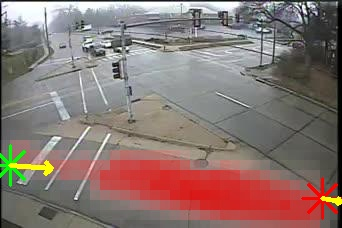
\includegraphics[width=\linewidth]{./img/scene_learning/res/243653/243653_h264_0-0.jpg}
        \end{subfigure}
        \begin{subfigure}{0.32\linewidth}
            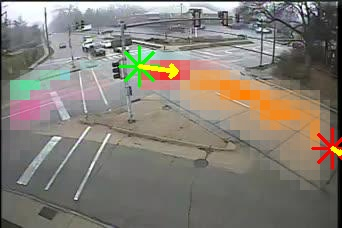
\includegraphics[width=\linewidth]{./img/scene_learning/res/243653/243653_h264_0-1.jpg}
        \end{subfigure}
        \begin{subfigure}{0.32\linewidth}
            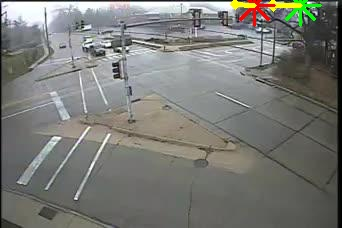
\includegraphics[width=\linewidth]{./img/scene_learning/res/243653/243653_h264_0-2.jpg}
        \end{subfigure}
        \caption{Failure case with simultaneous opposite directions. Entry (green) and exit (red) locations with direction (yellow arrows).}
        \label{fig:entry-exit-fail-1}
\end{figure}
\begin{figure}
    \centering
        \begin{subfigure}{0.32\linewidth}
            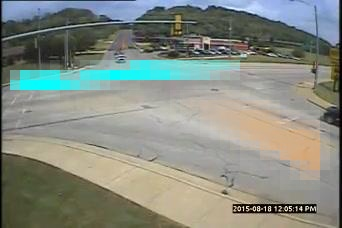
\includegraphics[width=\linewidth]{./img/scene_learning/res/251950/251950-0.jpg}
        \end{subfigure}
        \begin{subfigure}{0.32\linewidth}
            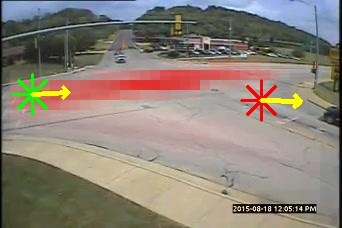
\includegraphics[width=\linewidth]{./img/scene_learning/res/251950/251950-1.jpg}
        \end{subfigure}

        \begin{subfigure}{0.32\linewidth}
            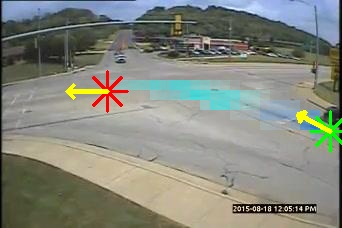
\includegraphics[width=\linewidth]{./img/scene_learning/res/251950/251950-2.jpg}
        \end{subfigure}
        \begin{subfigure}{0.32\linewidth}
            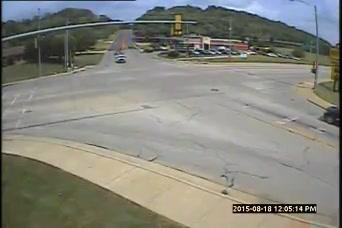
\includegraphics[width=\linewidth]{./img/scene_learning/res/251950/251950-3.jpg}
        \end{subfigure}
        \caption{Failure case with simultaneous opposite directions. Entry (green) and exit (red) with direction (yellow arrows) at a crowded intersection.}
        \label{fig:entry-exit-fail-2}
\end{figure}